\section{Results}
\label{sec:results}

\subsection{Mock classifier systematics}
\label{sec:mockresults}

Our first set of experiments investigates the relative responses of the log-loss and Brier metrics as a function of isolated systematic effects imposed on baselines of the best possible classifier.

\begin{figure}
	\begin{center}
		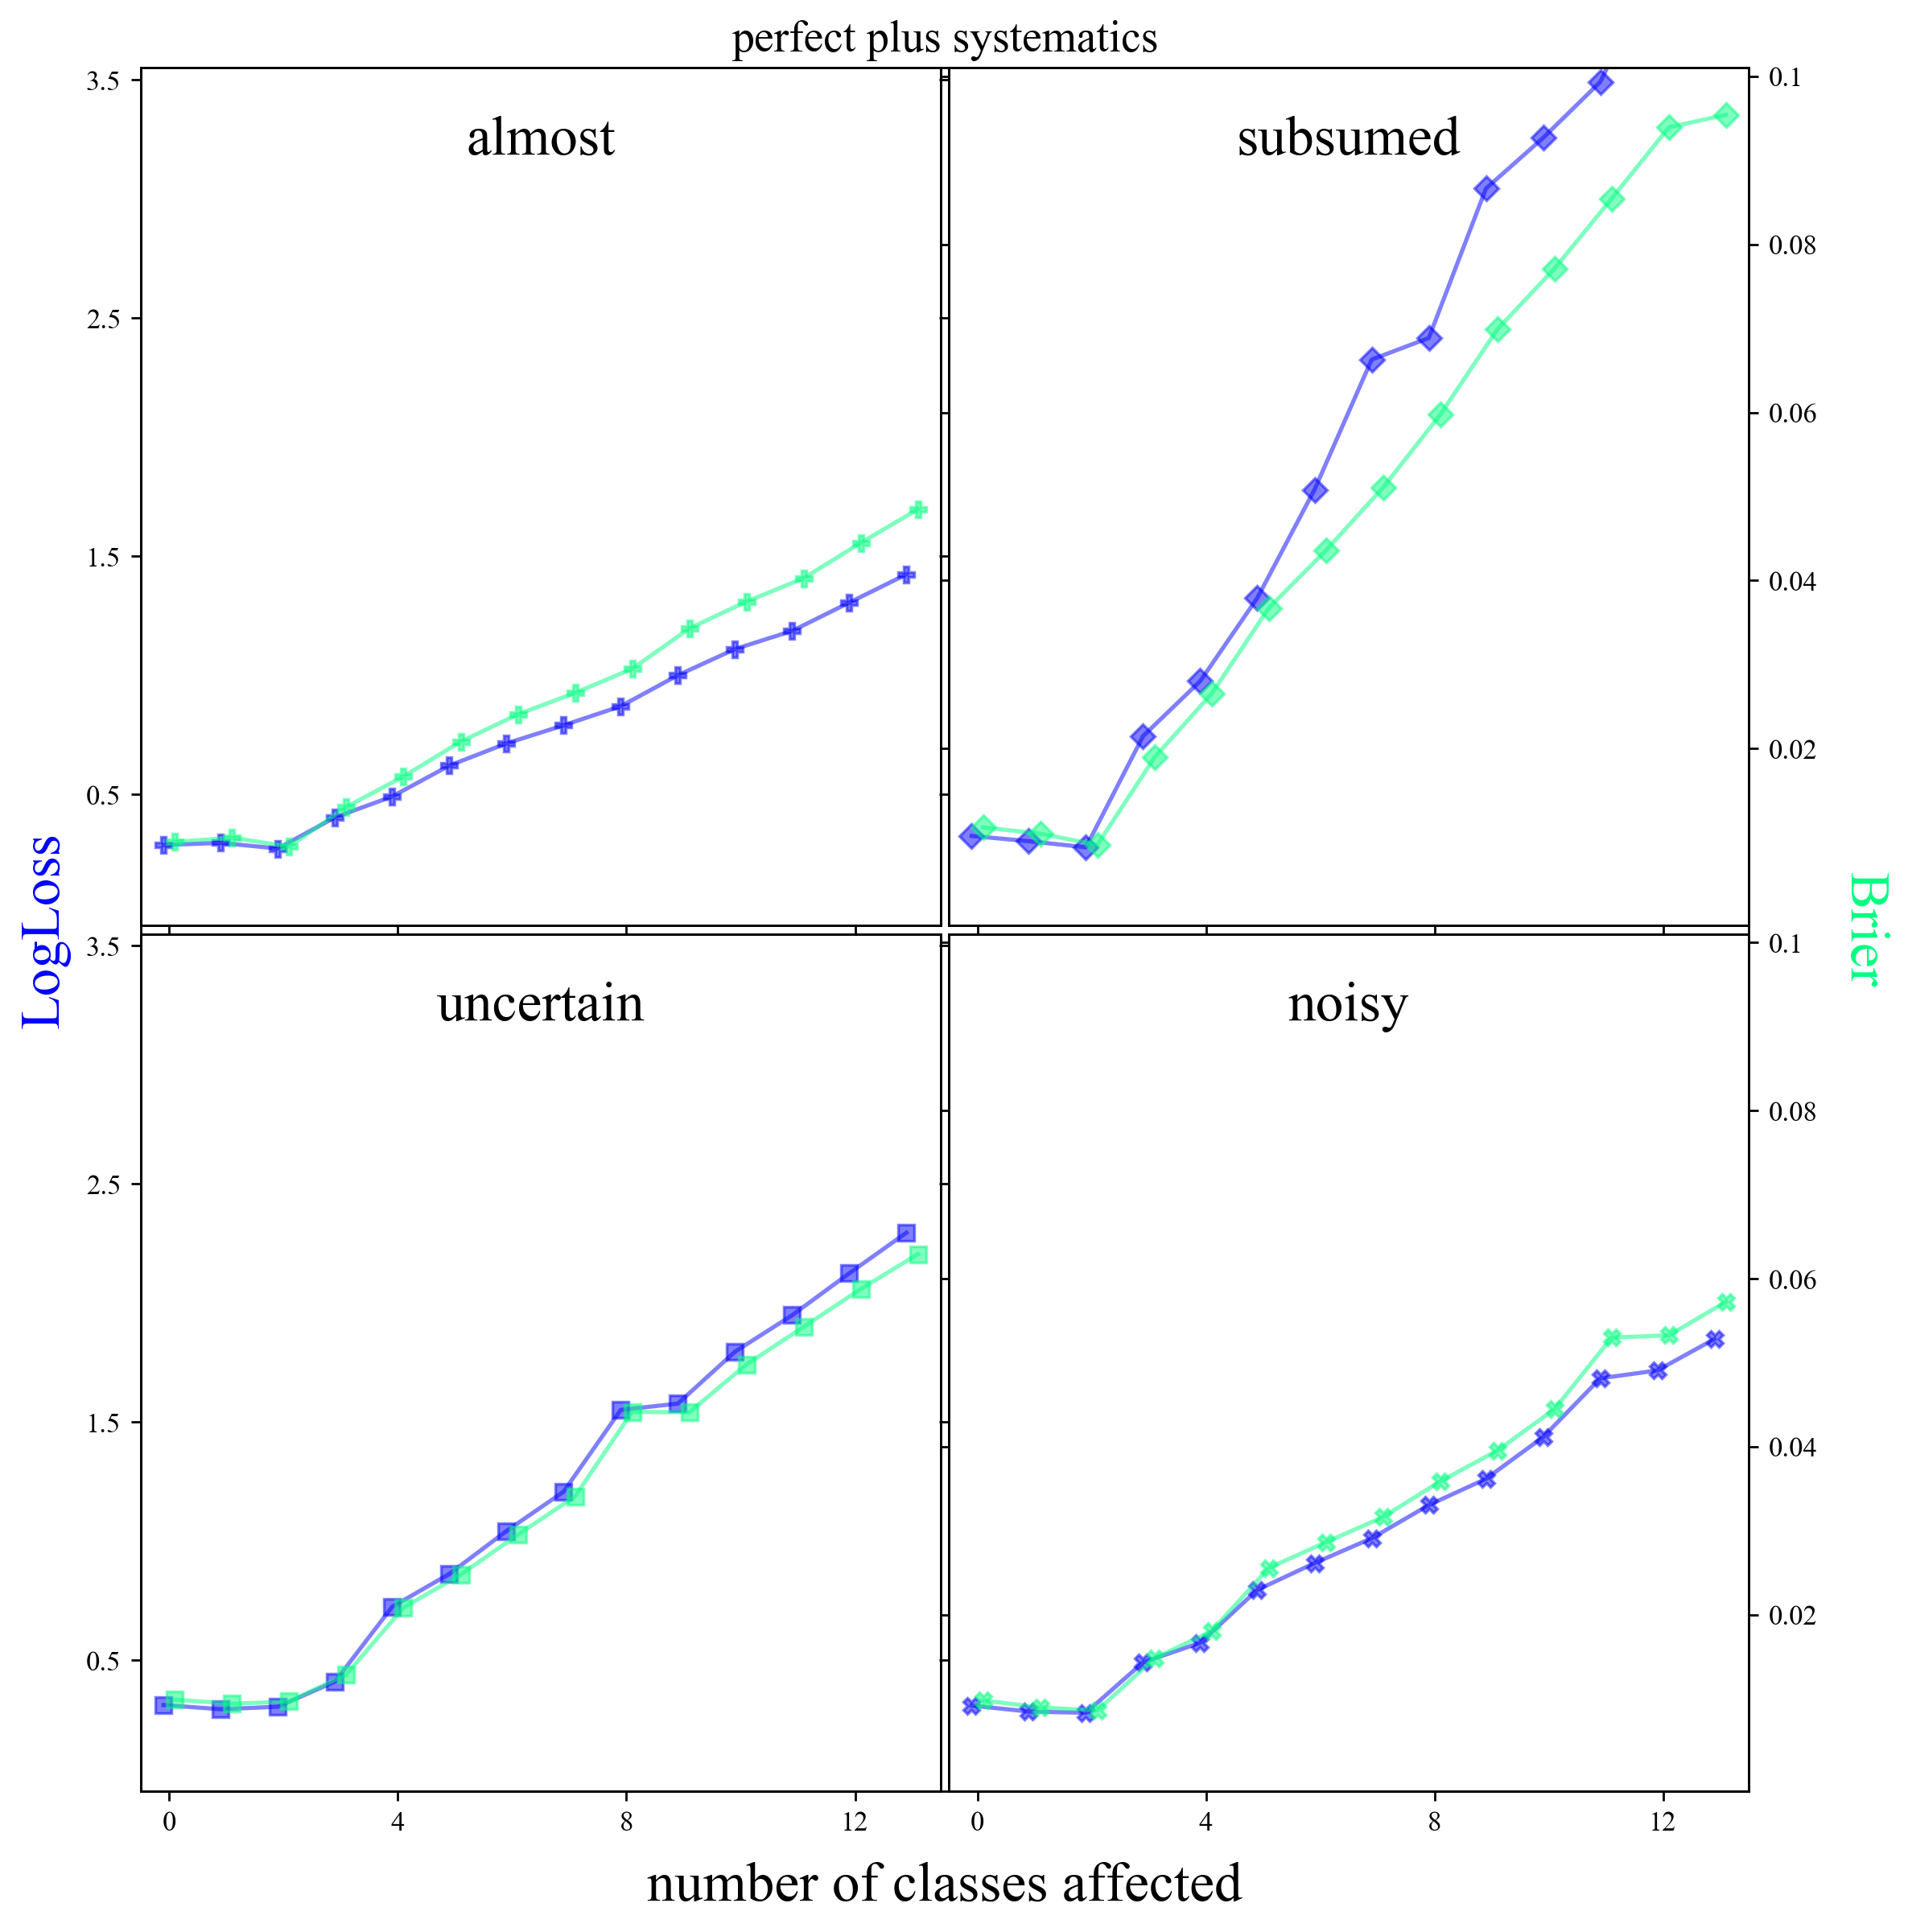
\includegraphics[width=0.5\textwidth]{./fig/systematics_onlyperfect.png}
		\caption{}
		\label{fig:subsume}
	\end{center}
\end{figure}

Figure~\ref{fig:subsume} shows the effect of adding each of four forms of error to a perfect classification, one class at a time, and calculating the metrics with flat weightings.
We confirm that more palatable effects affect the metric values in minor ways and those considered most severe have a more obvious effect.
Both metrics are appropriate for singling out a classifier that enables any class to subsume other classes.



\subsection{Representative classifications}
\label{sec:realresults}

\begin{figure*}
	\begin{center}
		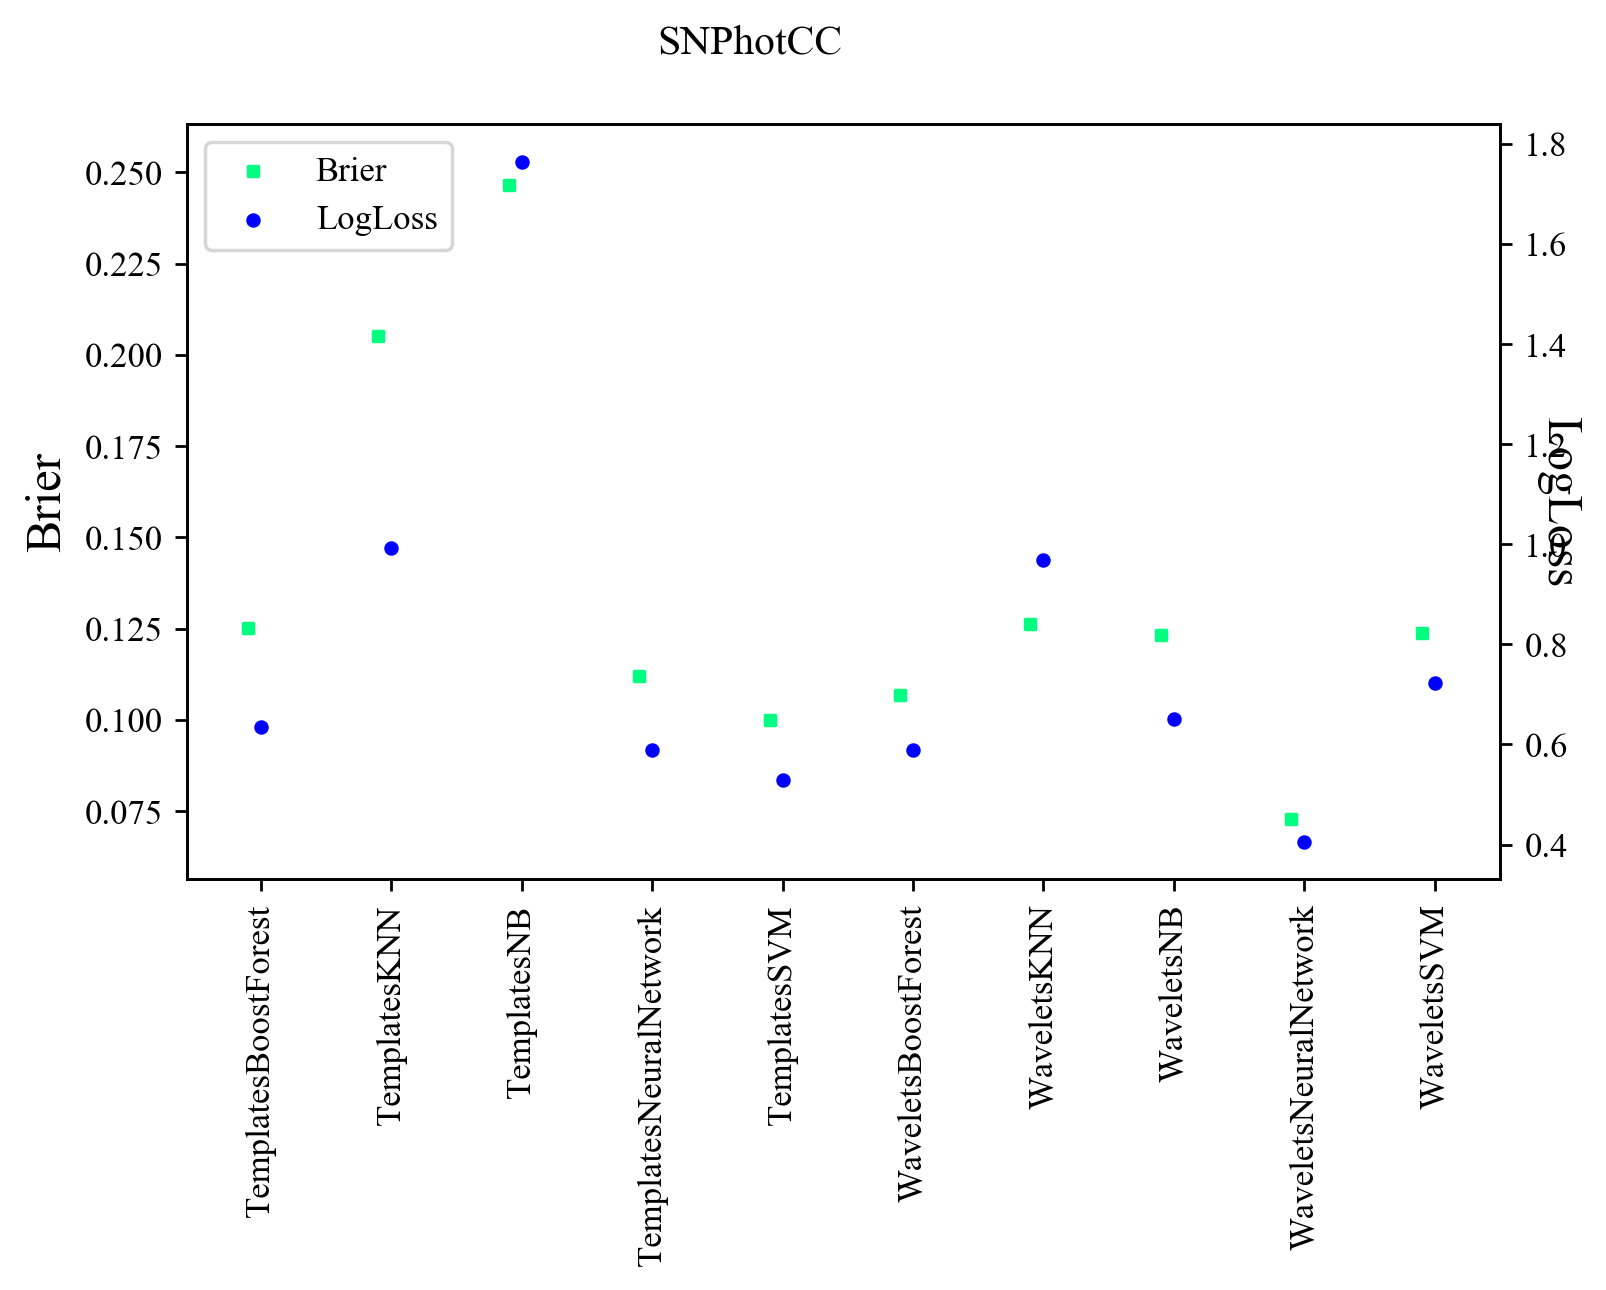
\includegraphics[width=0.45\textwidth]{./fig/SNPhotCC_res.png}
		% 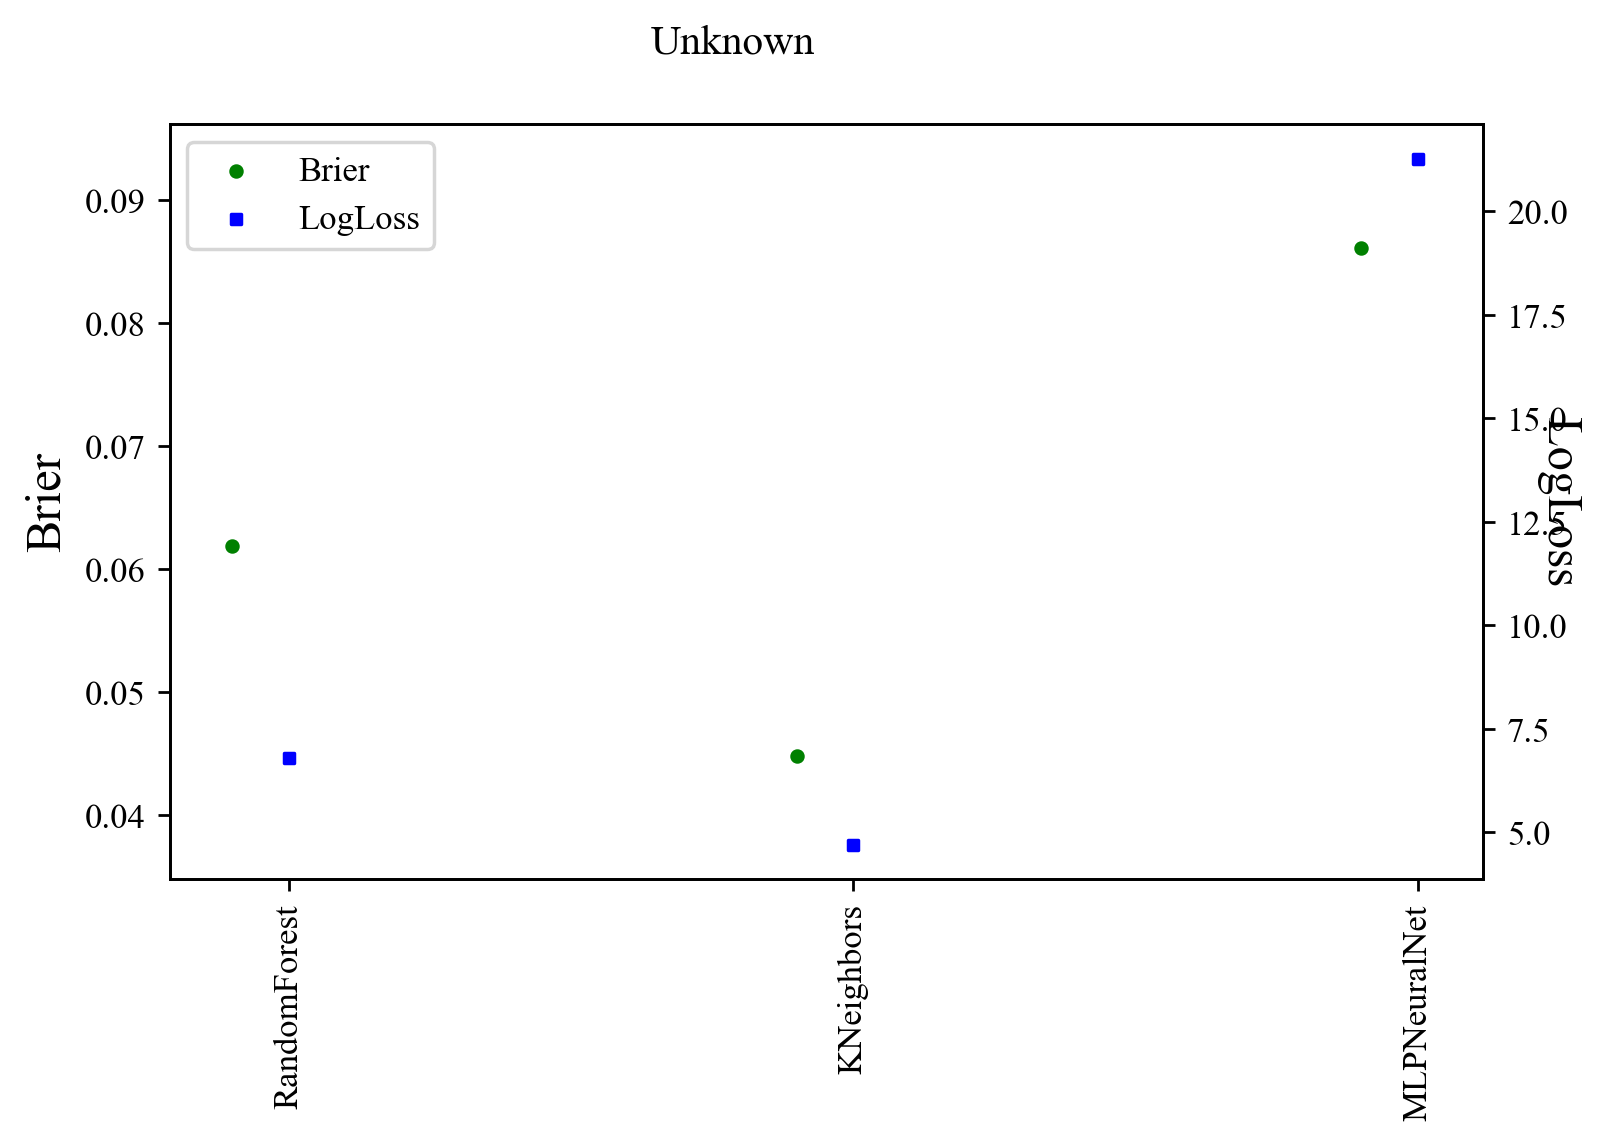
\includegraphics[width=0.45\textwidth]{./fig/Unknown_res.png}
		\caption{equal weight per class -- what kinds of weightings are meaningful to test here?  Would it be reasonable to take the real SNPhotCC entries' confusion matrices and see who would have won under each weighting/metric combination?}
		\label{fig:real_metric_compare}
	\end{center}
\end{figure*}

\subsection{Weighting systematics}
\label{sec:weight_res}

\aim{We have not yet reached consensus on what tests are reasonable in the absence of physical motivations, as the test cases here are independent of such context.}
% \begin{figure}
% 	\begin{center}
% 		% 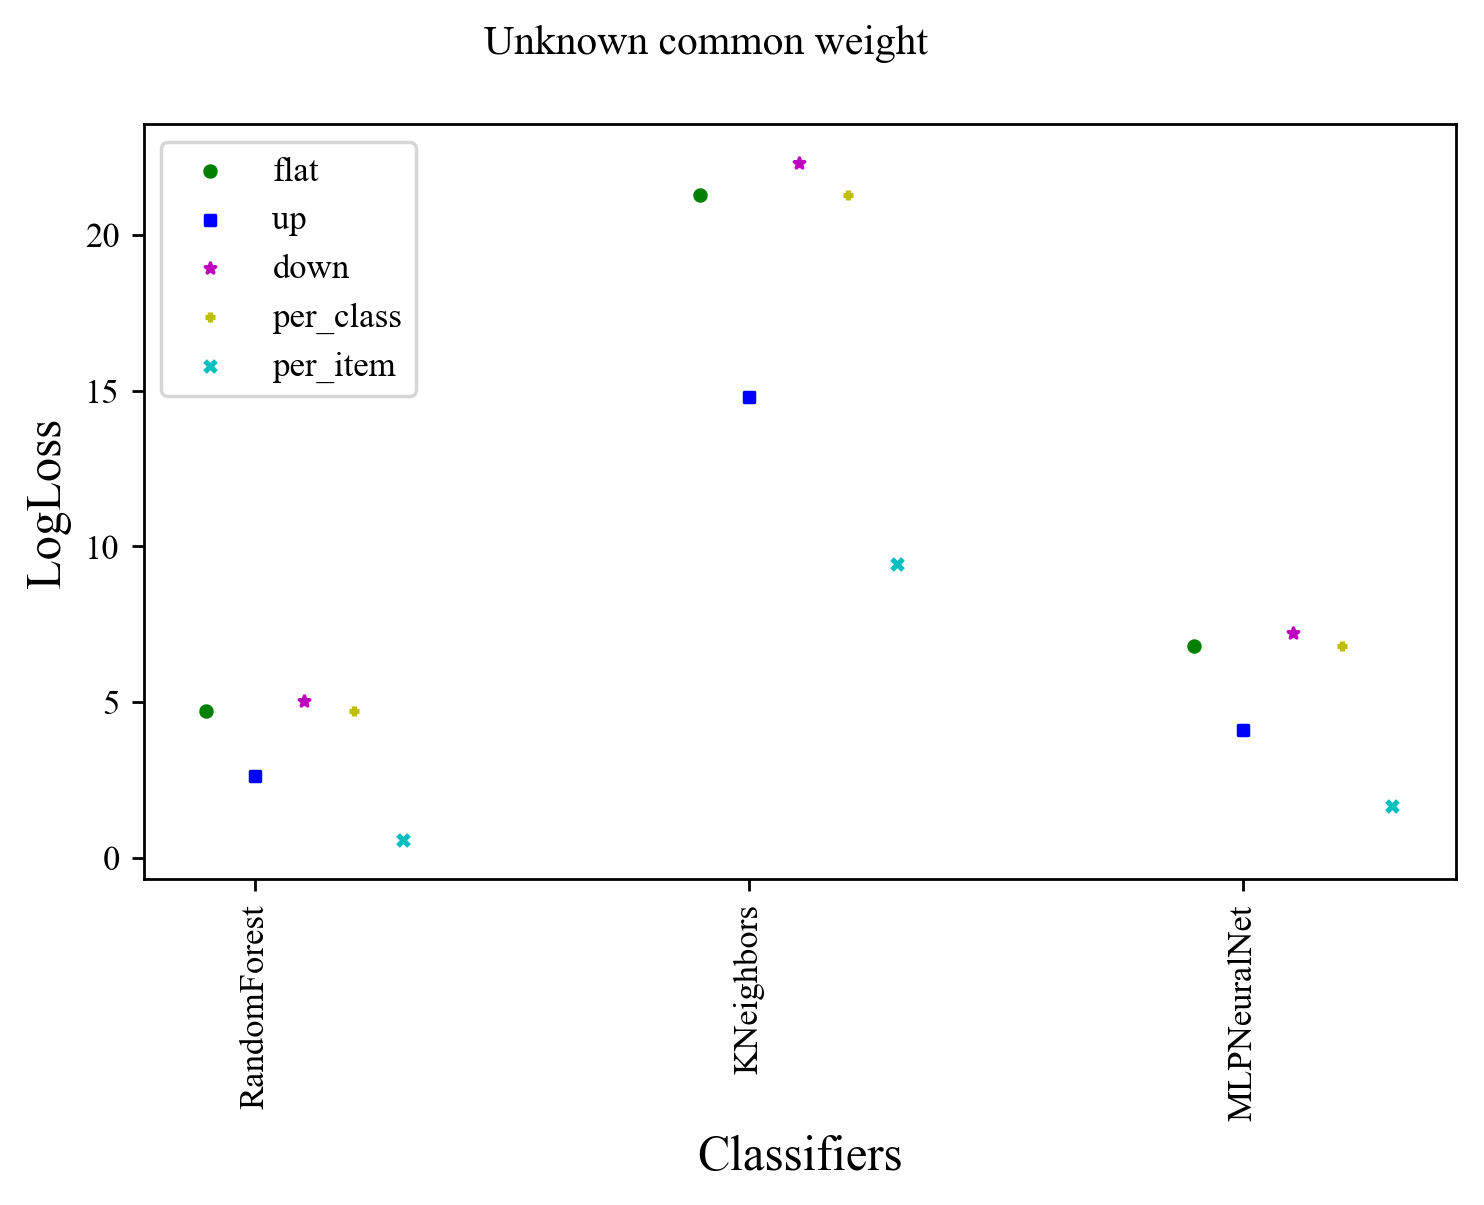
\includegraphics[width=0.5\textwidth]{./fig/systematic_Unknown_common.png}
% 		\caption{upweighting most common (best accuracy?)}
% 		\label{fig:systematic_common}
% 	\end{center}
% \end{figure}
%
% \begin{figure}
% 	\begin{center}
% 		% 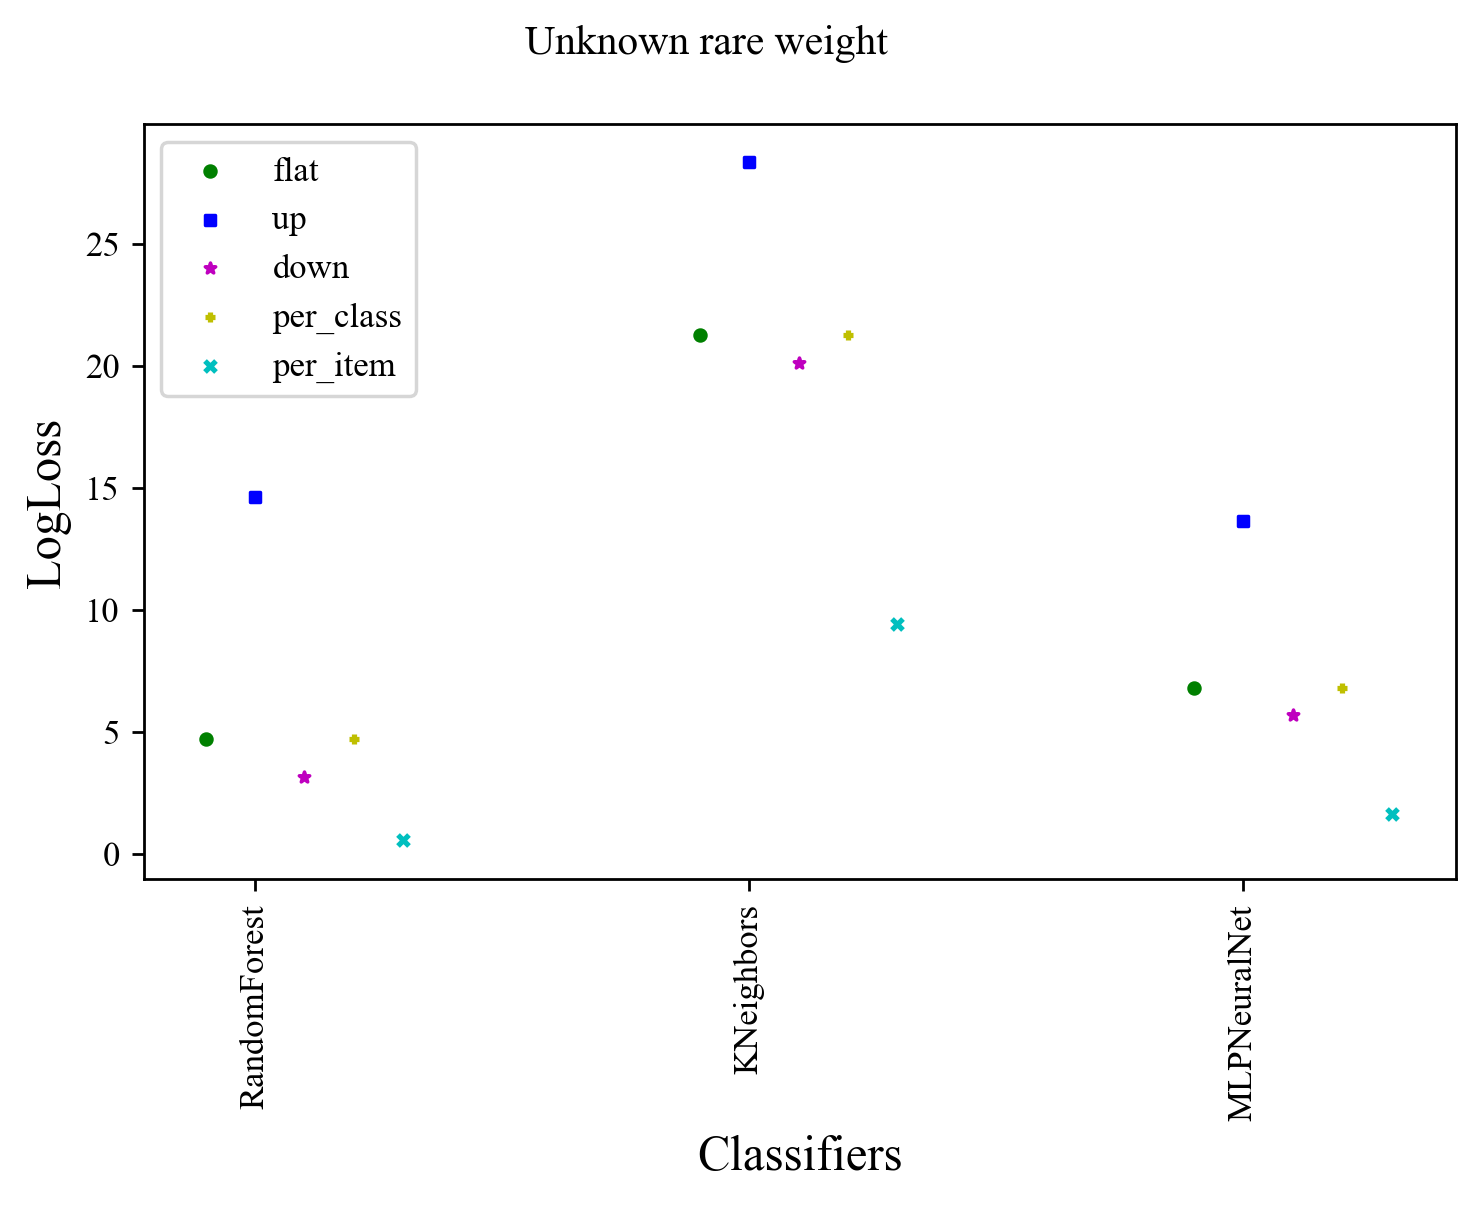
\includegraphics[width=0.5\textwidth]{./fig/systematic_Unknown_rare.png}
% 		\caption{upweighting least common (worst accuracy?)}
% 		\label{fig:systematic_rare}
% 	\end{center}
% \end{figure}
%
% \begin{figure}
% 	\begin{center}
% 		% 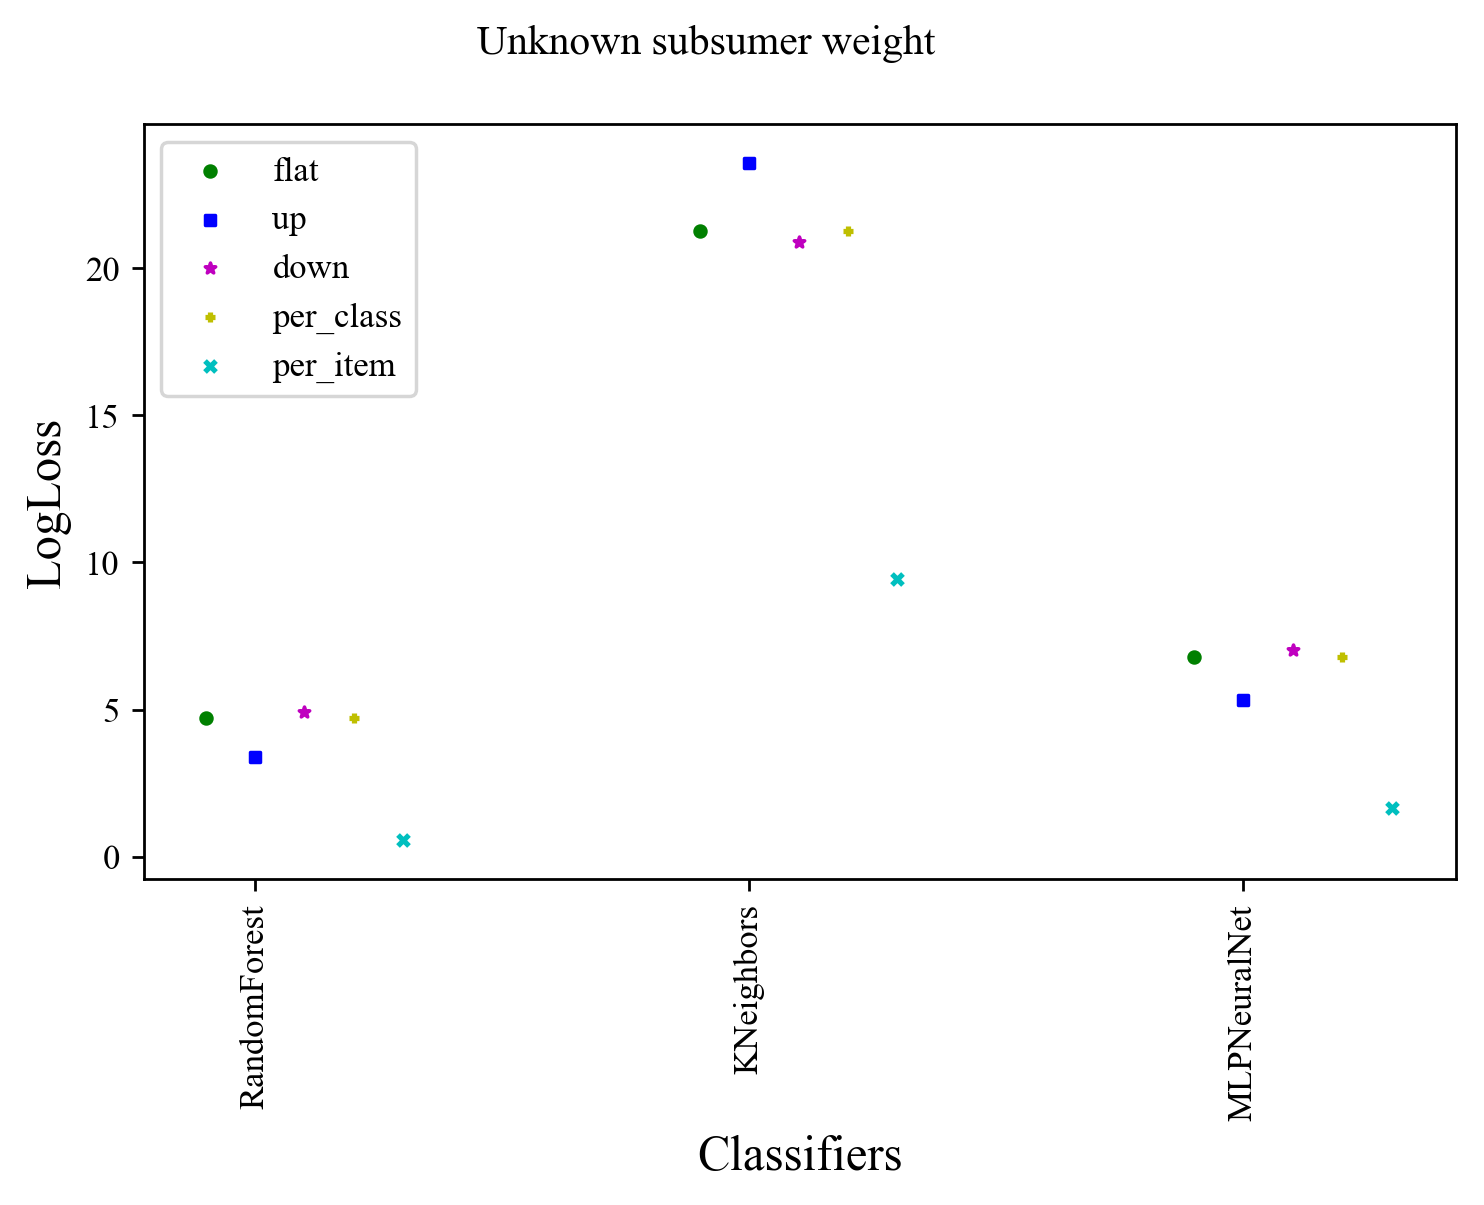
\includegraphics[width=0.5\textwidth]{./fig/systematic_Unknown_subsumer.png}
% 		\caption{upweighting class commonly misclassified as another class}
% 		\label{fig:systematic_subsumer}
% 	\end{center}
% \end{figure}
%
% \begin{figure}
% 	\begin{center}
% 		% 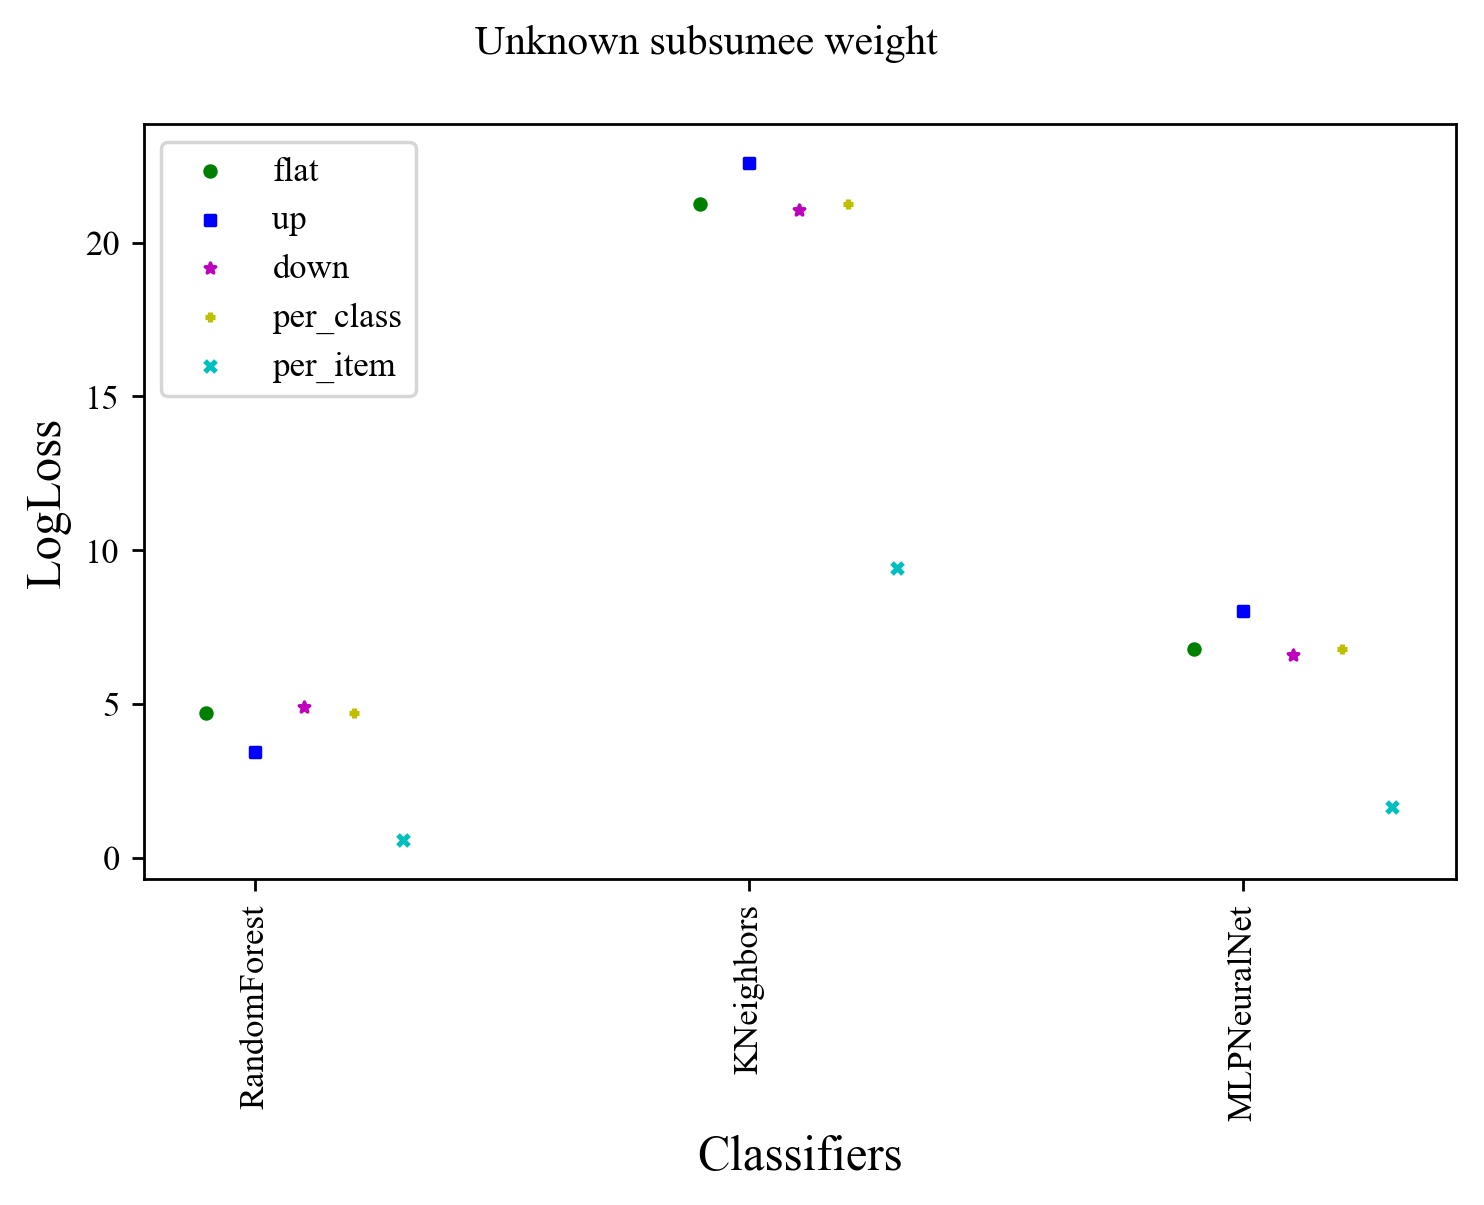
\includegraphics[width=0.5\textwidth]{./fig/systematic_Unknown_subsumee.png}
% 		\caption{upweighting class that a combination of other real classes are classified as}
% 		\label{fig:systematic_subsumee}
% 	\end{center}
% \end{figure}
%
% \begin{figure}
% 	\begin{center}
% 		% 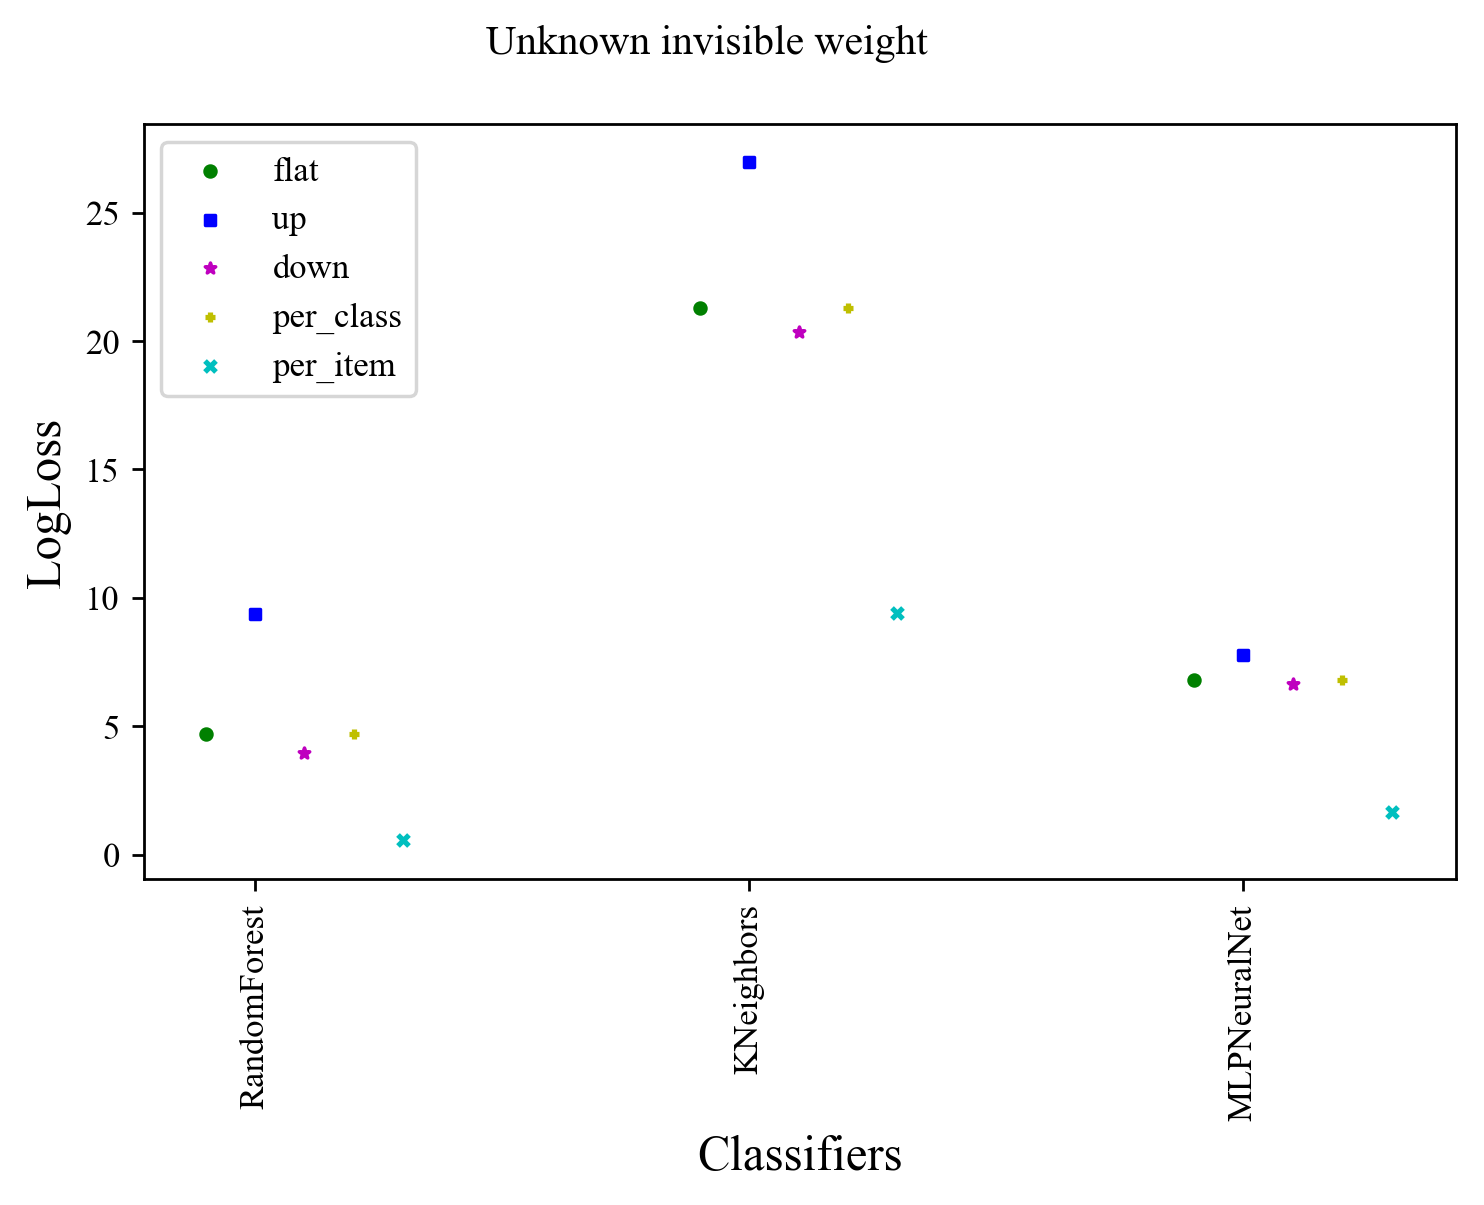
\includegraphics[width=0.5\textwidth]{./fig/systematic_Unknown_invisible.png}
% 		\caption{upweighting class that's totally missed}
% 		\label{fig:systematic_invisible}
% 	\end{center}
% \end{figure}
